\chapter{Zweiter Anhang - Ermittlung des PV-Ertrags anhand der Globalstrahlung}
\label{Kap:Anhang2}
Der Inhalt dieses Kapitels zeigt die Berechnung von PV-Erträgen bei senkrecht auf die Modulfläche eintreffender Globalstrahlung. Außerdem wird der Rechenweg für die Bestimmung des senkrecht auf eine geneigte Fläche treffende Globalstrahlung an der senkrecht auf den Grund eintreffenden Globalstrahlung gezeigt.

  \section{PV-Ertrag bei anhand senkrecht auf die Modulfläche eintreffender Globalstrahlung bestimmen}
      \label{Kap:PV_global}
      Die erzeugte DC-Leistung $P_{PV,DC}$ berechnet sich aus dem Wirkungsgrad $\eta_{PV}$ der Zellen, der Kollektorfläche $A$ und der senkrecht auf die geneigte Modulfläche treffende Globalstrahlung $G_{0,g}$ mit der Kollektorfläche $A$.
	
      \begin{equation}
          P_{PV,DC} = \eta_{PV} \cdot G_{0,g} \cdot A
          \label{Eq:PV_Pdc}
      \end{equation}

      Der Wirkungsgrad $\eta_{PV}$ kann anhand der Peakleistung $P_p$ bestimmt werden.

      \begin{equation}
          \eta_{PV} = \frac{\frac{P_p}{A}}{G_{STC}} = \frac{\frac{P_p}{A}}{1000 \frac{W}{m^2}}
          \label{Eq:PV_eta}
      \end{equation}

      Die Ausgangsleistung des PV-Wechselrichters $P_{PV,AC}$ wird wie folgt berechnet.

      \begin{equation}
          P_{PV,AC} = \eta_{WR} \cdot P_{PV} = \eta_{WR} \cdot \eta_{PV} \cdot G_{0,g} \cdot A
          \label{Eq:PV_Pac}
      \end{equation}

	\section{Bestimmung der senkrecht auf eine geneigte Modulfläche eintreffenden Globalstrahlung}	
    	\label{Kap:G0g}
		Die vertikal auf eine geneigte Modulfläche eintreffende Globalstrahlung $G_{0,g}$ kann anhand der senkrecht auf den Grund treffenden Globalstrahlung $G_0$ gemäß Gleichung \ref{Eq:G0g} und \ref{Eq:cospsi} mit den in Tabelle \ref{Tab:sonnenwinkel} sowie den Abbildungen \ref{Abb:sonnenwinkel1} und \ref{Abb:sonnenwinkel2} definierten Winkelgrößen bestimmt werden.\cite{REN2}
        
      \begin{equation}
          G_{0,g} = G_0 \cdot cos(\psi)	
          \label{Eq:G0g}
      \end{equation}
      mit der Kosinusfunktion des Einfallswinkels $\psi$ nach folgender Gleichung:
      \begin{multline}
          cos(\psi) = (cos(\alpha) sin(\Phi) - sin(\alpha) cos(\Phi) cos(\beta)) sin(\delta) + \\
          ((cos(\alpha) cos(\Phi) + sin(\alpha) sin(\Phi) cos(\beta)) cos(\delta) cos(t) + \\ 
          sin(\alpha) sin(\beta) cos(\delta) sin(t) 
          \label{Eq:cospsi}
      \end{multline}

      "Die Deklination $\delta$ schwankt aufgrund der scheinbaren Sonnenbewegung um $\pm 23,450 {^\circ}$"\cite{REN2} und kann folgendermaßen berechnet werden, wobei d der Tag des Jahres, vom 1. Januar aus gezählt ist: \\ 
      \begin{equation}
          \delta = -23,45^{\circ} \cdot cos(360^{\circ} /365,25^{\circ} (d+10)) 
      \end{equation}

      Der Stundenwinkel t lässt sich aus der Rotationsgeschwindigkeit der Erde ermitteln.
      \begin{equation}
          15\degree/h (12h - WOZ) ~\text{dabei ist}~ WOZ = GZ + 4 min \cdot (\lambda_0 - \lambda) - Z
      \end{equation} 
      $ \text{und } Z/min = -7,66 sin(x) - 9,87 sin( 2x + 24,99\degree + 3,83\degree sin(x))$ \\
      $ \text{mit }x = 0,9856\degree d-2,72\degree$ \\

      Die wahre Ortszeit WOZ (Sonnenzeit) kann sich von der gesetzlich geregelten Zeit GZ (Ortszeit) je nach Ortslage und Jahreszeit unterscheiden. Die Ortszeit ist auf einen Längenmeridian $\lambda_0$ bezogen (z.B. MEZ: Bezungsmeridian $\lambda_0 = -15\degree$). \\
	
	
	\begin{table}[h]
		\begin{tabular}{|c|l|} %ggf. Mitte auch zentrieren
			\hline 
			Zeichen & Definition \\ 
			\hline 
			$\alpha \quad[$\degree$] $ & Neigungswinkel (gegen Horizontale)  \\ 
			\hline 
			$\beta \quad [$\degree$] $ & Azimutwinkel (Ost-West-Orientierung) (Empfangsfläche) \\ 
			\hline 
			$\delta \quad [$\degree$] $ & Deklination, Winkelabstand des Sonnenhöchststands vom Himmelsäquator  \\ 
			\hline 
			$\lambda \quad [$\degree$] $ & geographische Länge (Meridian)  \\ 
			\hline
			$\psi \quad [$\degree$] $ & Einfallswinkel (zwischen Strahlungsrichtung \& Flächennormalen)  \\ 
			\hline 
			$\Phi \quad [$\degree$] $ & geographische Breite  \\ 
			\hline 
			$t \quad [$\degree$] $ & Stundenwinkel (Sonnenstand) \\ 
			\hline 
		\end{tabular} 
		\caption{Beschreibung der Winkel um die Position der Erde zur Sonne zu beschreiben}
		\label{Tab:sonnenwinkel}
	\end{table}

\begin{landscape}
	\begin{figure}[h]
		\centering
		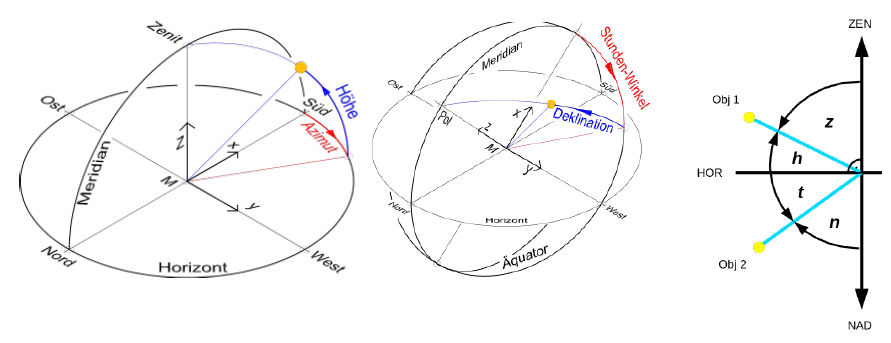
\includegraphics[width=\linewidth]{Strahlungswinkel_Sonne1}
		\caption{Relevante beschreibende Winkelgrößen, welche die Bewegung der Erde um die Sonne beschreiben und so für $G_{0,g}$ entscheidend sind. Die Variablen des Horizonts- und des Äquator-Koordinatensystems (links und mittig). Rechts die Aufteilung im Horizont-Koordinatensystem für die nördliche (Zenit) und südliche (Nadir) Halbkugel.\cite{REN2}}
		\label{Abb:sonnenwinkel1}
	\end{figure}
	
	\begin{figure}[h]
		\centering
		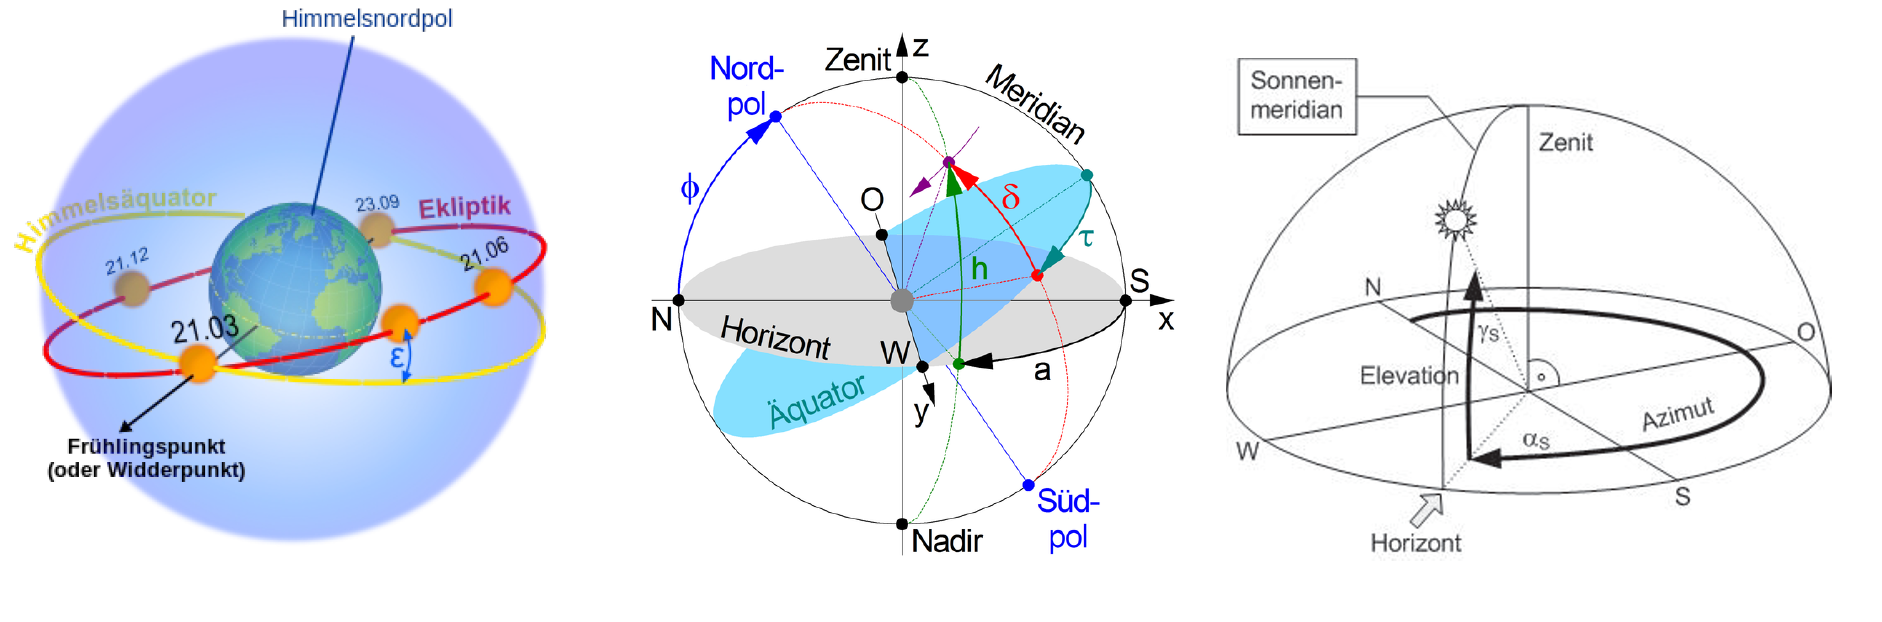
\includegraphics[width=\linewidth]{Strahlungswinkel_Sonne2}
		\caption{Relevante beschreibende Winkelgrößen, welche die Bewegung der Erde um die Sonne beschreiben und so für $G_{0,g}$ entscheidend sind. Hier Ekliptik und Himmelsäquator bzw. Horizont \cite{REN2}}
		\label{Abb:sonnenwinkel2}
	\end{figure}
\end{landscape}
        